\documentclass[a4paper,12pt]{article}

\usepackage[T1]{fontenc}
\usepackage{amsmath}
\usepackage[
    backend=biber,
    style=authoryear,
    sorting=nyt
]{biblatex}
\usepackage{kvsetkeys}
\addbibresource{/references.bib}
\title{Competition structure optimization (Project 5)}
\author{Leonard Hell and Klara Resch}
\date{\today}

\begin{document}

\maketitle
\section{Introduction}
For the multiobjective Optimization we chose the following Problem. We consider a competition with n participants and we want to optimize the competition structure. We consider a given strength distribution among the participants and the following structure.
\begin{figure}[htbp]
    \centering
    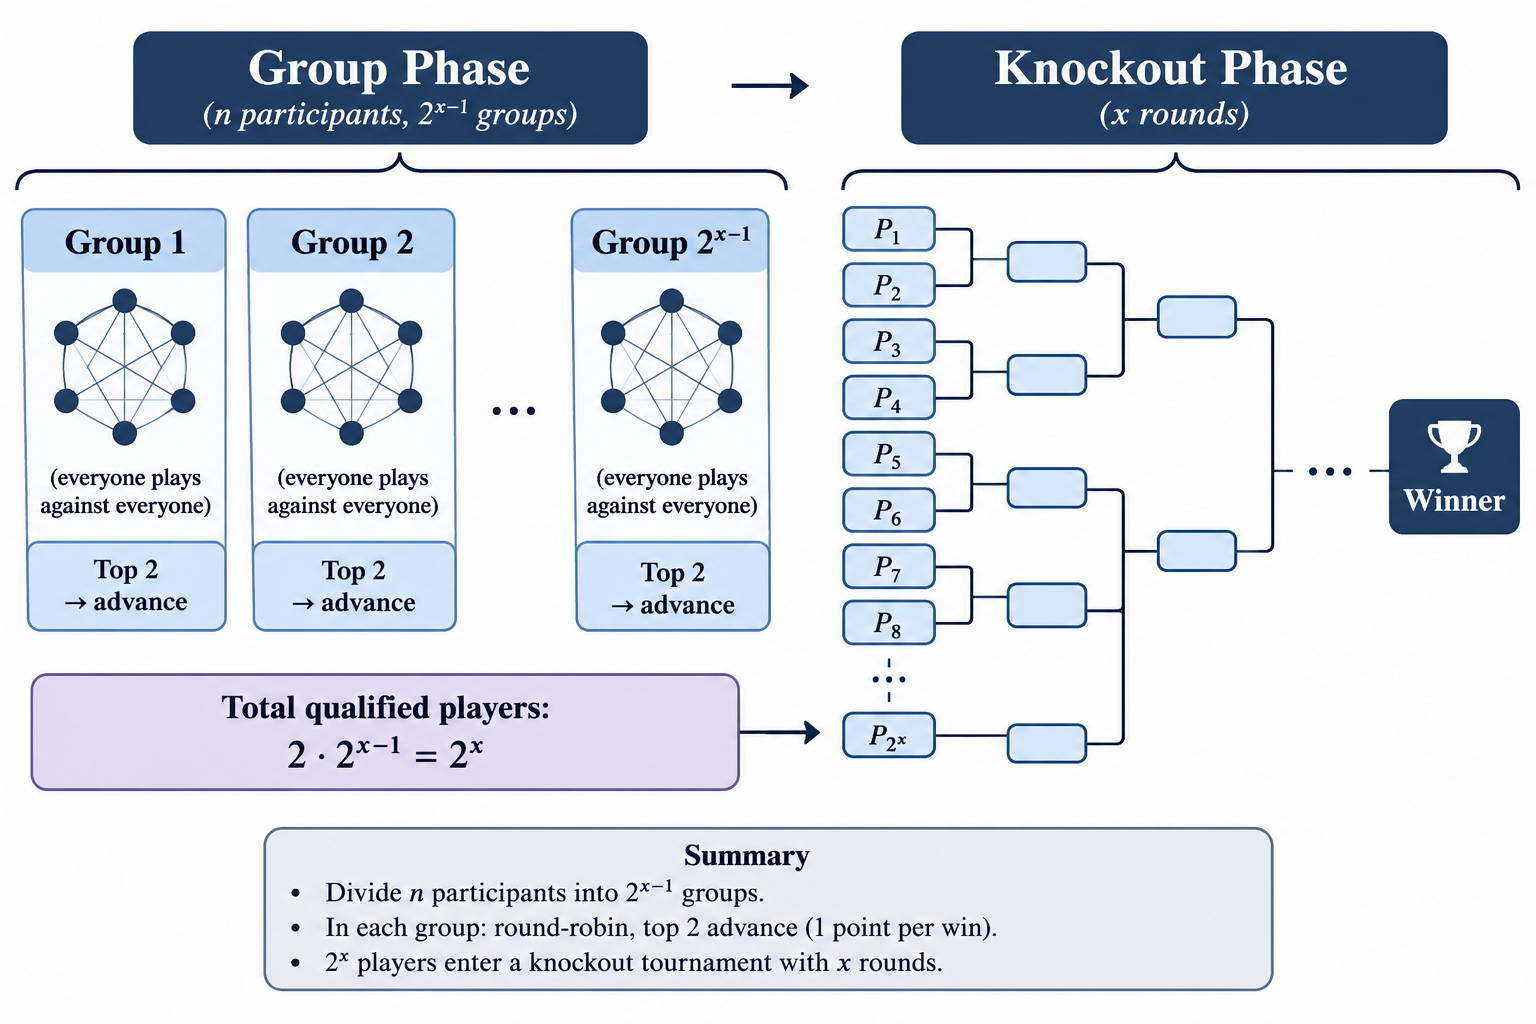
\includegraphics[width=0.9\textwidth]{Gruppen- und K.-o.-Turnierformat.png}
    \caption{Schematic representation of the competition structure.}
    \label{fig:competition-structure}
\end{figure}
 We want to minimize number of games in total, maximize the probability that the strongest player wins and maximze the suspense i.e. that the result is unpredictable.
 Blablabla mathe

 \section{Competition structure Problem}
 We consider $n$ players and generate the strength uniformly from 0 to 10. For the group phase (if there is one i.e.$ x < log_2(n)$) we divide the players into $2^{x-1}$ groups by snake seeding, so starting from the strongest player distributing one to each group and than going backwards.
\begin{align}
    n &= 4 \\
    \text{strength} &= \{0:0.9, 1:0.7, 2:0.5, 3:0.1\}
\end{align}
\begin{table}[htbp]
    \centering
    \begin{tabular}{c|c}
        group 1 & group 2 \\ \hline
        0       & 1       \\
        3       & 2
    \end{tabular}
    \caption{Example of group allocation}
    \label{tab:group-allocation}
\end{table}

\newpage
\printbibliography[title={References}]
\end{document}
